\documentclass[report.tex]{subfiles}

\externaldocument{report}

\begin{document}

\section{失敗点・言い訳・改善・頑張ったからほめてほしいところ ・その他} \label{sec:失敗点}

\subsection{アンテナの作成}

\subsubsection{かご}

まず、ループアンテナを作成するときに、\wfig{kago}のような100円ショップで買ったかごを巻き付けて作成しようと思った。
しかし、かごが斜めになっていたので両面テープを用いて補強しても巻き付けた部分がどうしてもズレてしまい、作業が進まなかった。
様々な巻数で電波の受信感度を測定できたらいいのではないかと思い、かごにドリルで穴を開けてそこから導線を通してみようと考えた。
しかし、そう思った時点では、すでにかなりの巻数を巻いてしまっていたので、全てほどかなければいけないことになってしまった。
かごの上の部分が少し出っ張っているので、ドリルで穴を開けるときに非常に困難であったり、穴を想定よりかなりズレたところに開けてしまったりした。
また、コイルが斜めっていると、アンテナ(インダクタンス)が想定していたものとは異なったりしてうまく機能しないのではないかと言われた(かごが斜めっていると、直径が変化してしまうため、計算がズレる)。
これらの失敗が重なり合ってしまって、かごに巻きつけてループアンテナを作成することを断念した。

\begin{figure}[H]
	\centering
	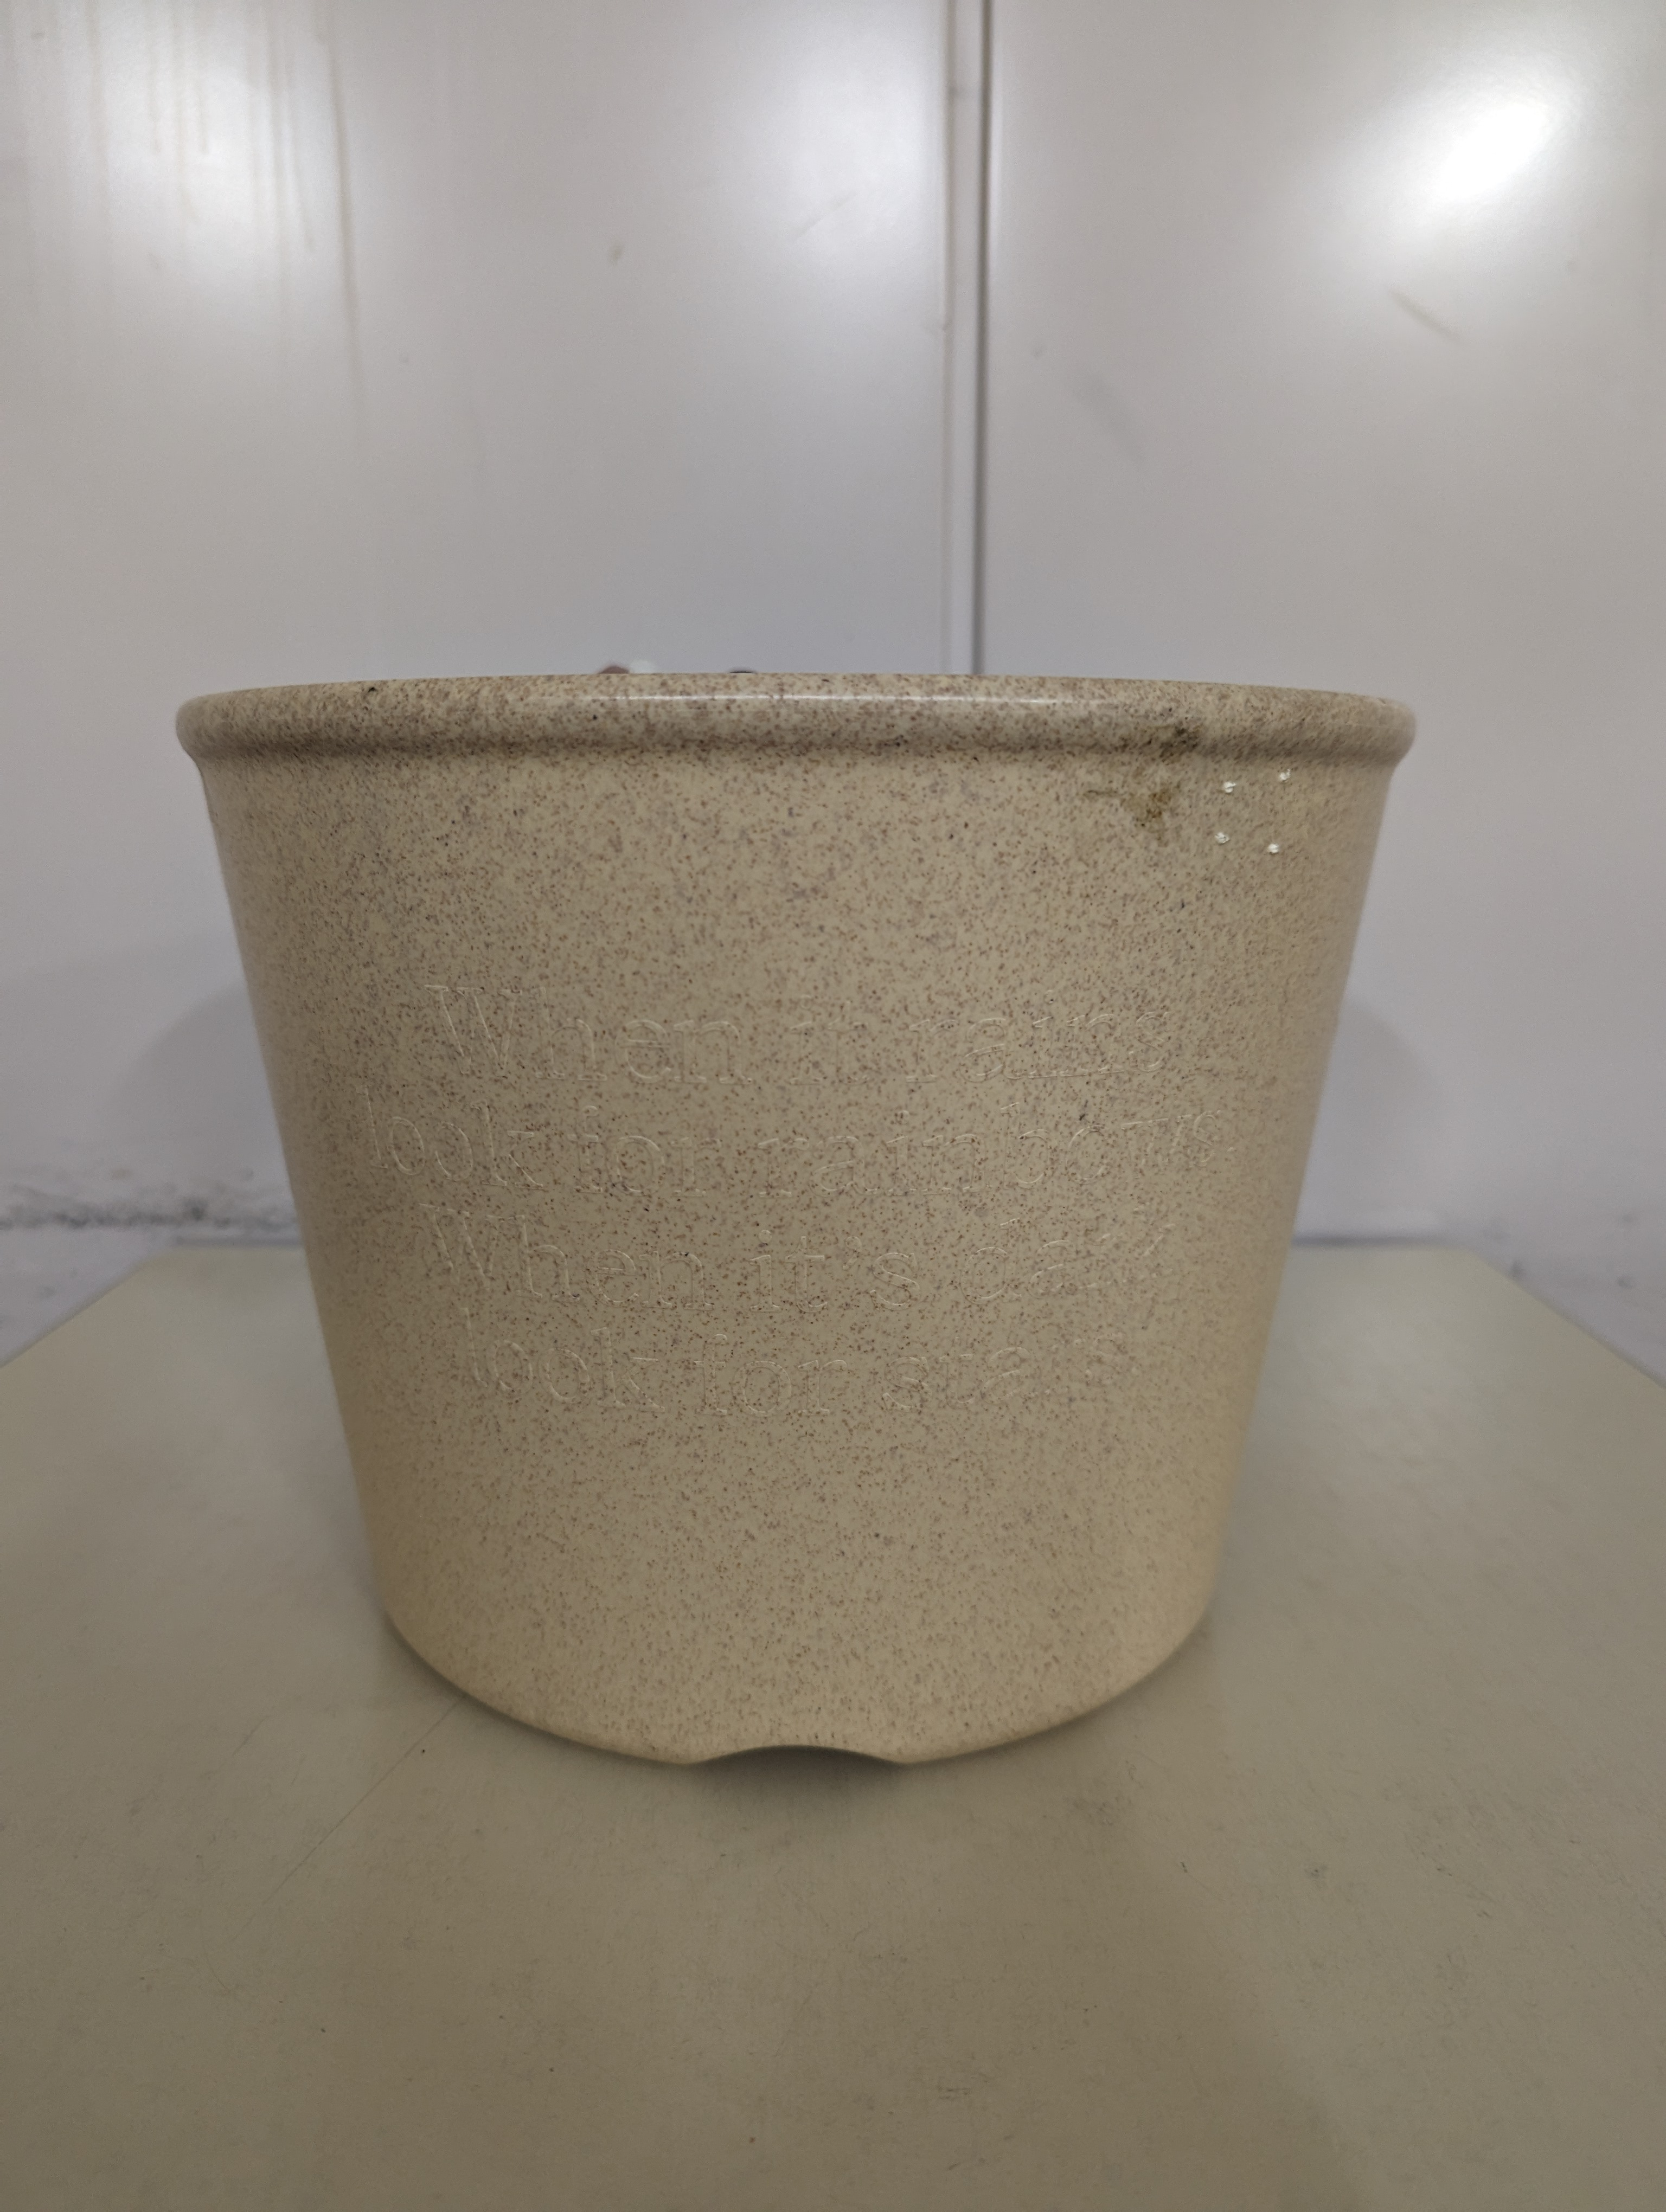
\includegraphics[width=7cm]{use/kago.jpg}
	\caption{かご}
	\label{fig:kago}
\end{figure}

\subsubsection{エナメル線}

最初に、0.32mmの導線でアンテナを巻き付ける際に、秋葉原で売っていた20mのエナメル線を用いた。
袋を開けてから、何も考えずにすぐに巻き付けようとしてしまった。
そのせいで導線がどんどんと絡まってしまった。
開封したての時は、きれいに巻かれていた導線だったため、引っ張れば一本の絡まっていない銅線になると勘違いしてしまった。
他の二人は引っ張るのは良くないと言っていたが、気づいたときには、元には戻せないほど絡まってしまった。
何とか元に戻そうとして、多くの時間をかけてほどこうとしたが、途中で銅線が切れてしまい、使い物にならなくなってしまった。
最終的に、機材室に置いてあった銅線を用いた。
機材室に置いてあったものは、すでに何かに巻かれてあるものであったため、少しずつほどきながら巻き付けていった。
そのため、絡まることなくアンテナを作成することができた。

\subsubsection{アンテナ一号機}

最終的に100円ショップに売ってあった画用紙を丸めて、ループアンテナを作成した。
しかし、画用紙がかなり柔らかかったため、巻きつける時に銅線がゆるくなってしまい、巻きつけるのに苦労してしまった。
また、画用紙の下半分(巻いていないところ)が長くて邪魔であったため、銅線を巻くのが困難で一周巻くのに1分ぐらいかかってしまった。
早く画用紙の下半分を切ってしまったほうが良かったと後悔した(いまだに切ってない)。
ループアンテナを巻く作業が最終的に3日ぐらいかかってしまった(失敗含めないで)。
そのため、画用紙に巻くのをいったん中断しなければいけないことになった。
機材室に置いてあった銅線に繋がったまま中断することになったが、機材室の人に機材室の奥の方で置かせてもらったので良かった。
また、作業するときに机も貸してもらった。
画用紙を用いて作ったループアンテナ(アンテナ一号機)のインダクタンスを調べるときに画用紙が柔らかかったせいで、軽く押しただけで特性が変化してしまった。
そのため、もう少し硬いものを用いて作成すればよかったと思った。
最終的に余った画用紙を丸めて、それを詰めることによってある程度形が安定したが、それでもインダクタンスが多少変化してしまった。
画用紙を詰めるのではなく、ペットボトルを詰めて作成すればよかったと思った。

\subsection{フィルタ回路の作成}

別の班が作成していた高い音と低い音をカットするローパスフィルターとハイパスフィルターの回路を参考にして、ノイズや発振をカットしてくれるアクティブフィルタの作成をしてもらった。
しかし、フェムトファラッド単位のコンデンサが必要になり、作業が難航した。
何とか頑張って\wfig{filter}のような回路を作成してもらった。
しかし、電源を用いて回路を作動させたところ、電源が短絡してしまっていた。
結局のところ原因がわからず、フィルタ回路を作成することはできなかった。

\subsubsection{アンテナ二号機}

アンテナ二号機は、ペットボトルに巻きつけて作成した。
ペットボトルは、アンテナ一号機の画用紙よりも硬くて、巻きつけるのが非常に楽だった(その分、直径が小さいため、たくさん巻かなければいけなくなった)。
アンテナ二号機の巻数を計算するために、定規で直径を測定した(7cmだった)。
ペットボトルのインダクタンスを測定して気づいたのだが、ペットボトルの直径は正確には少し小さかった(6.5cmだった)。
計算してみると、長さが0.5cm違うだけで、

\begin{figure}[H]
	\centering
	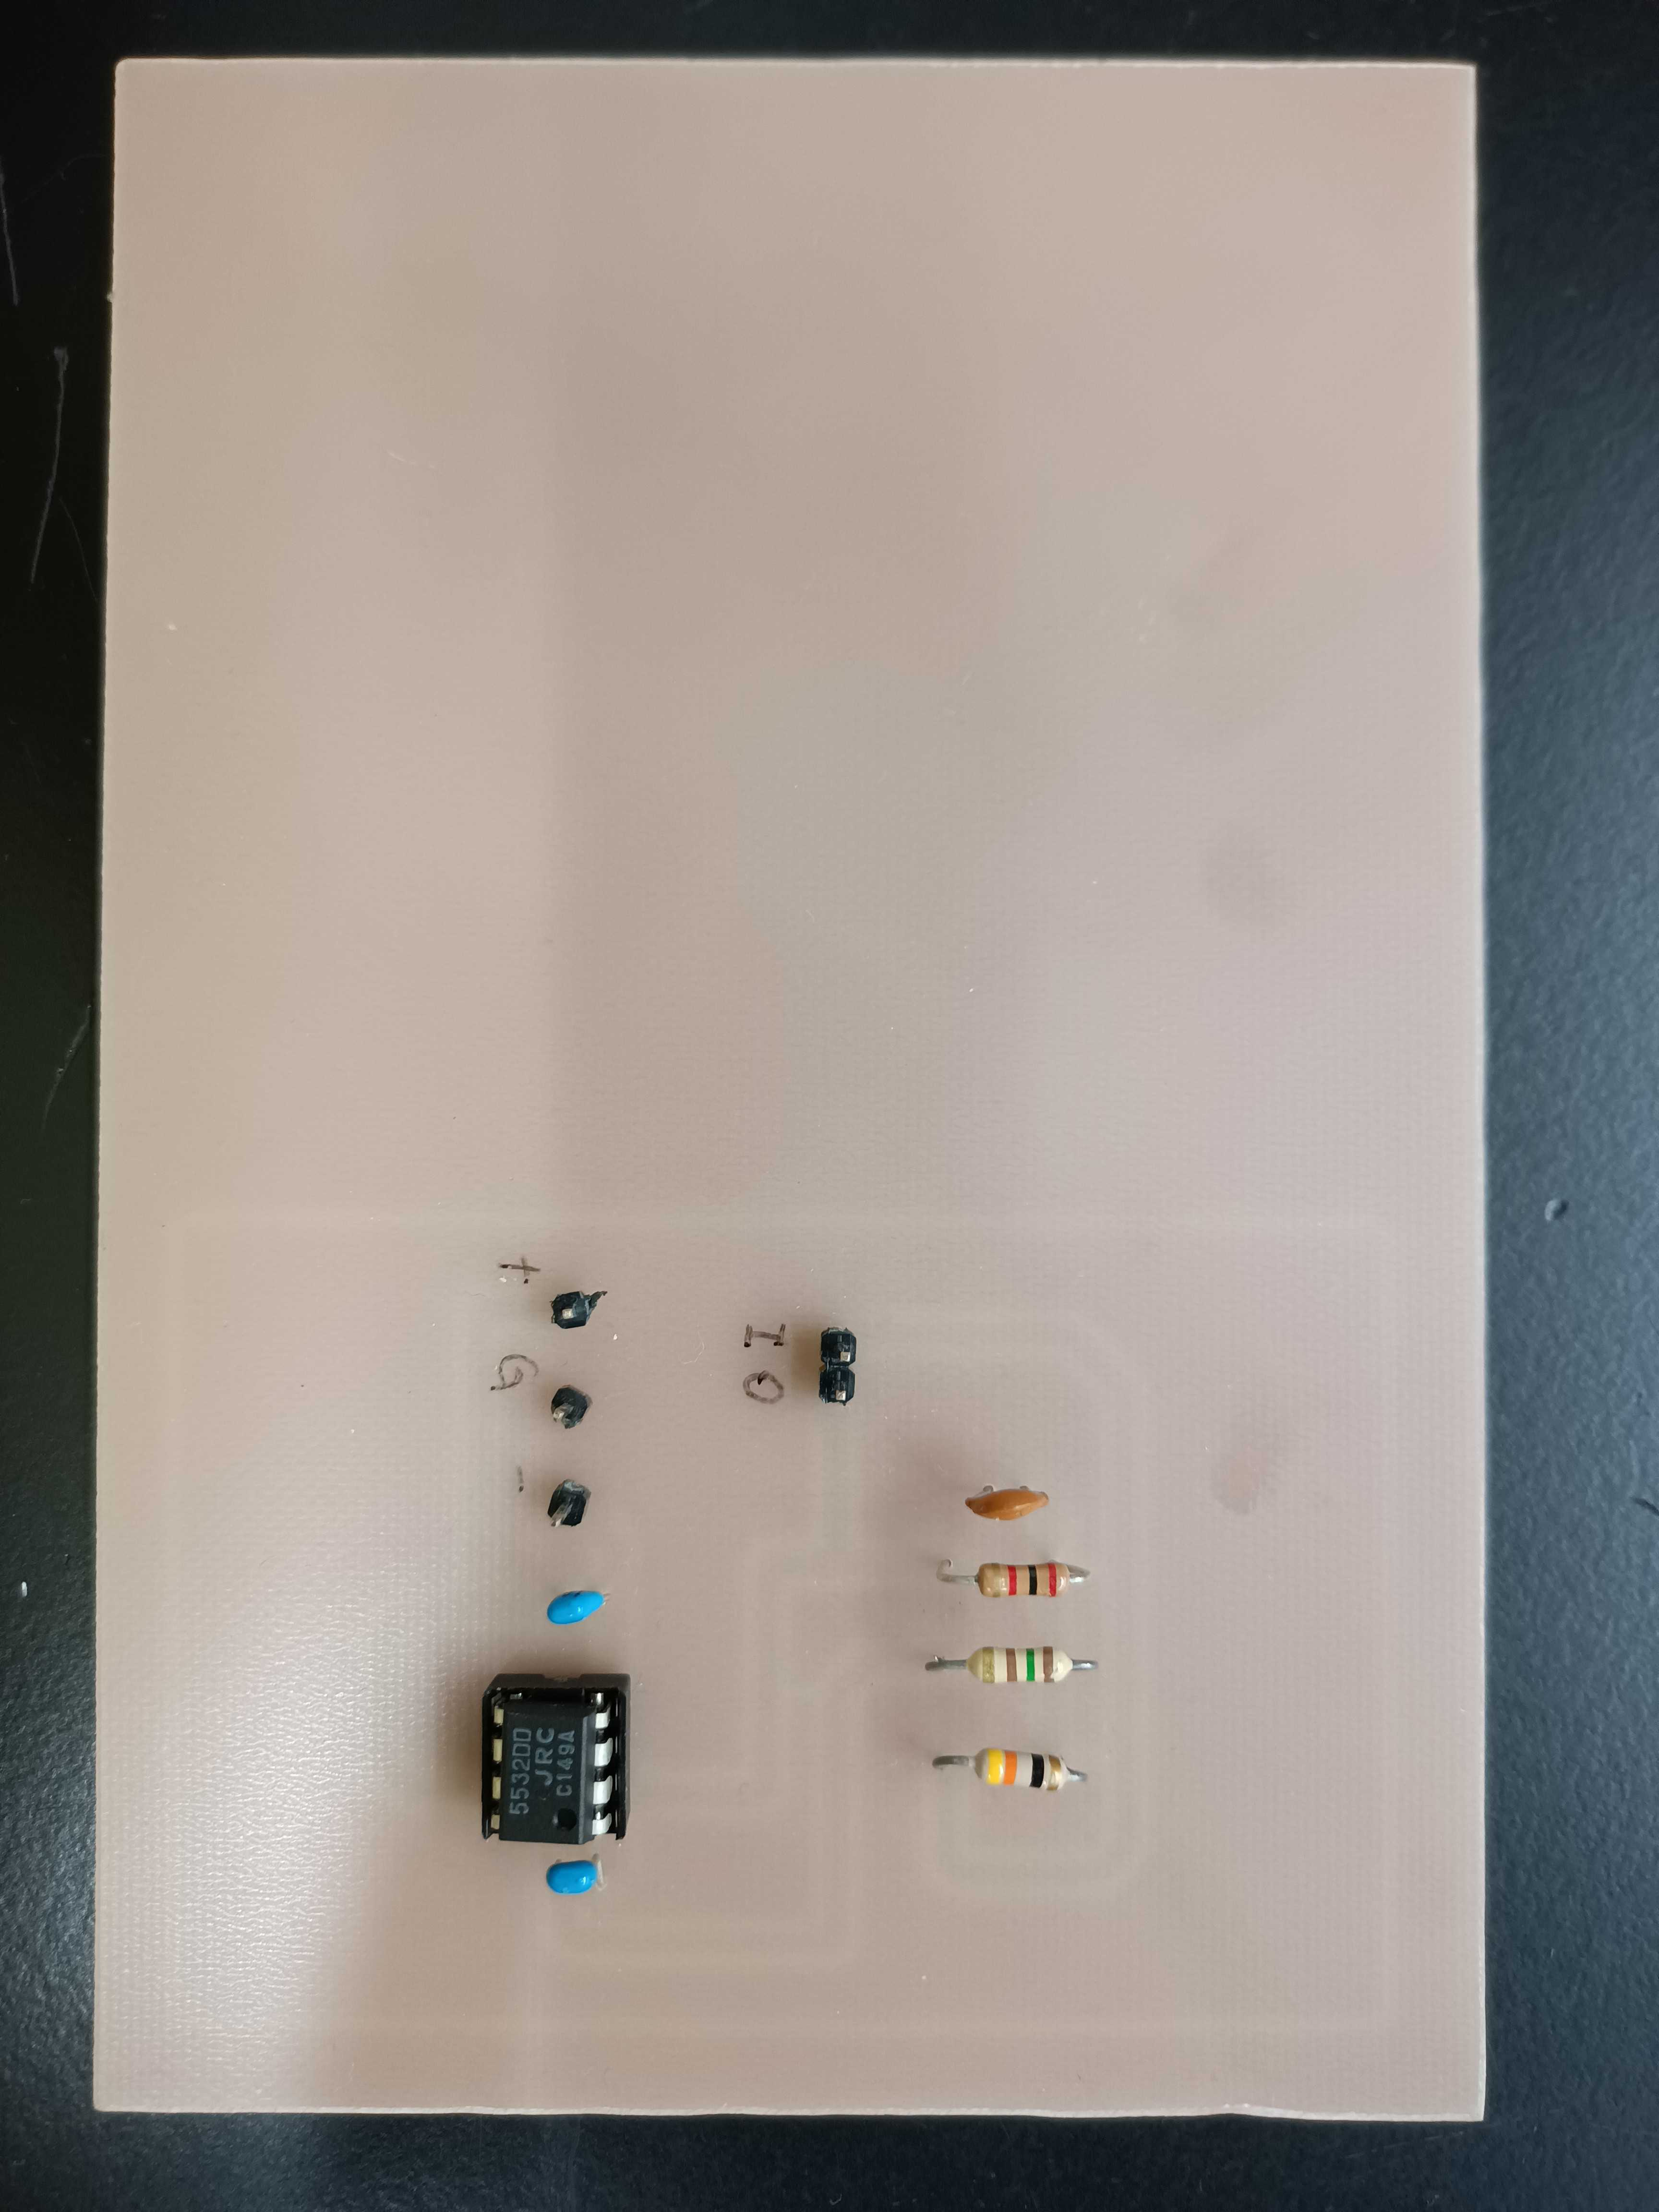
\includegraphics[width=7cm]{use/1.jpg}
	\caption{フィルタ回路}
	\label{fig:filter}
\end{figure}

\subsection{増幅回路の作成}

\wfig{s_2}にアンプ一台目を示す。

\begin{figure}[H]
	\begin{minipage}[b]{0.5\linewidth}
		\centering
		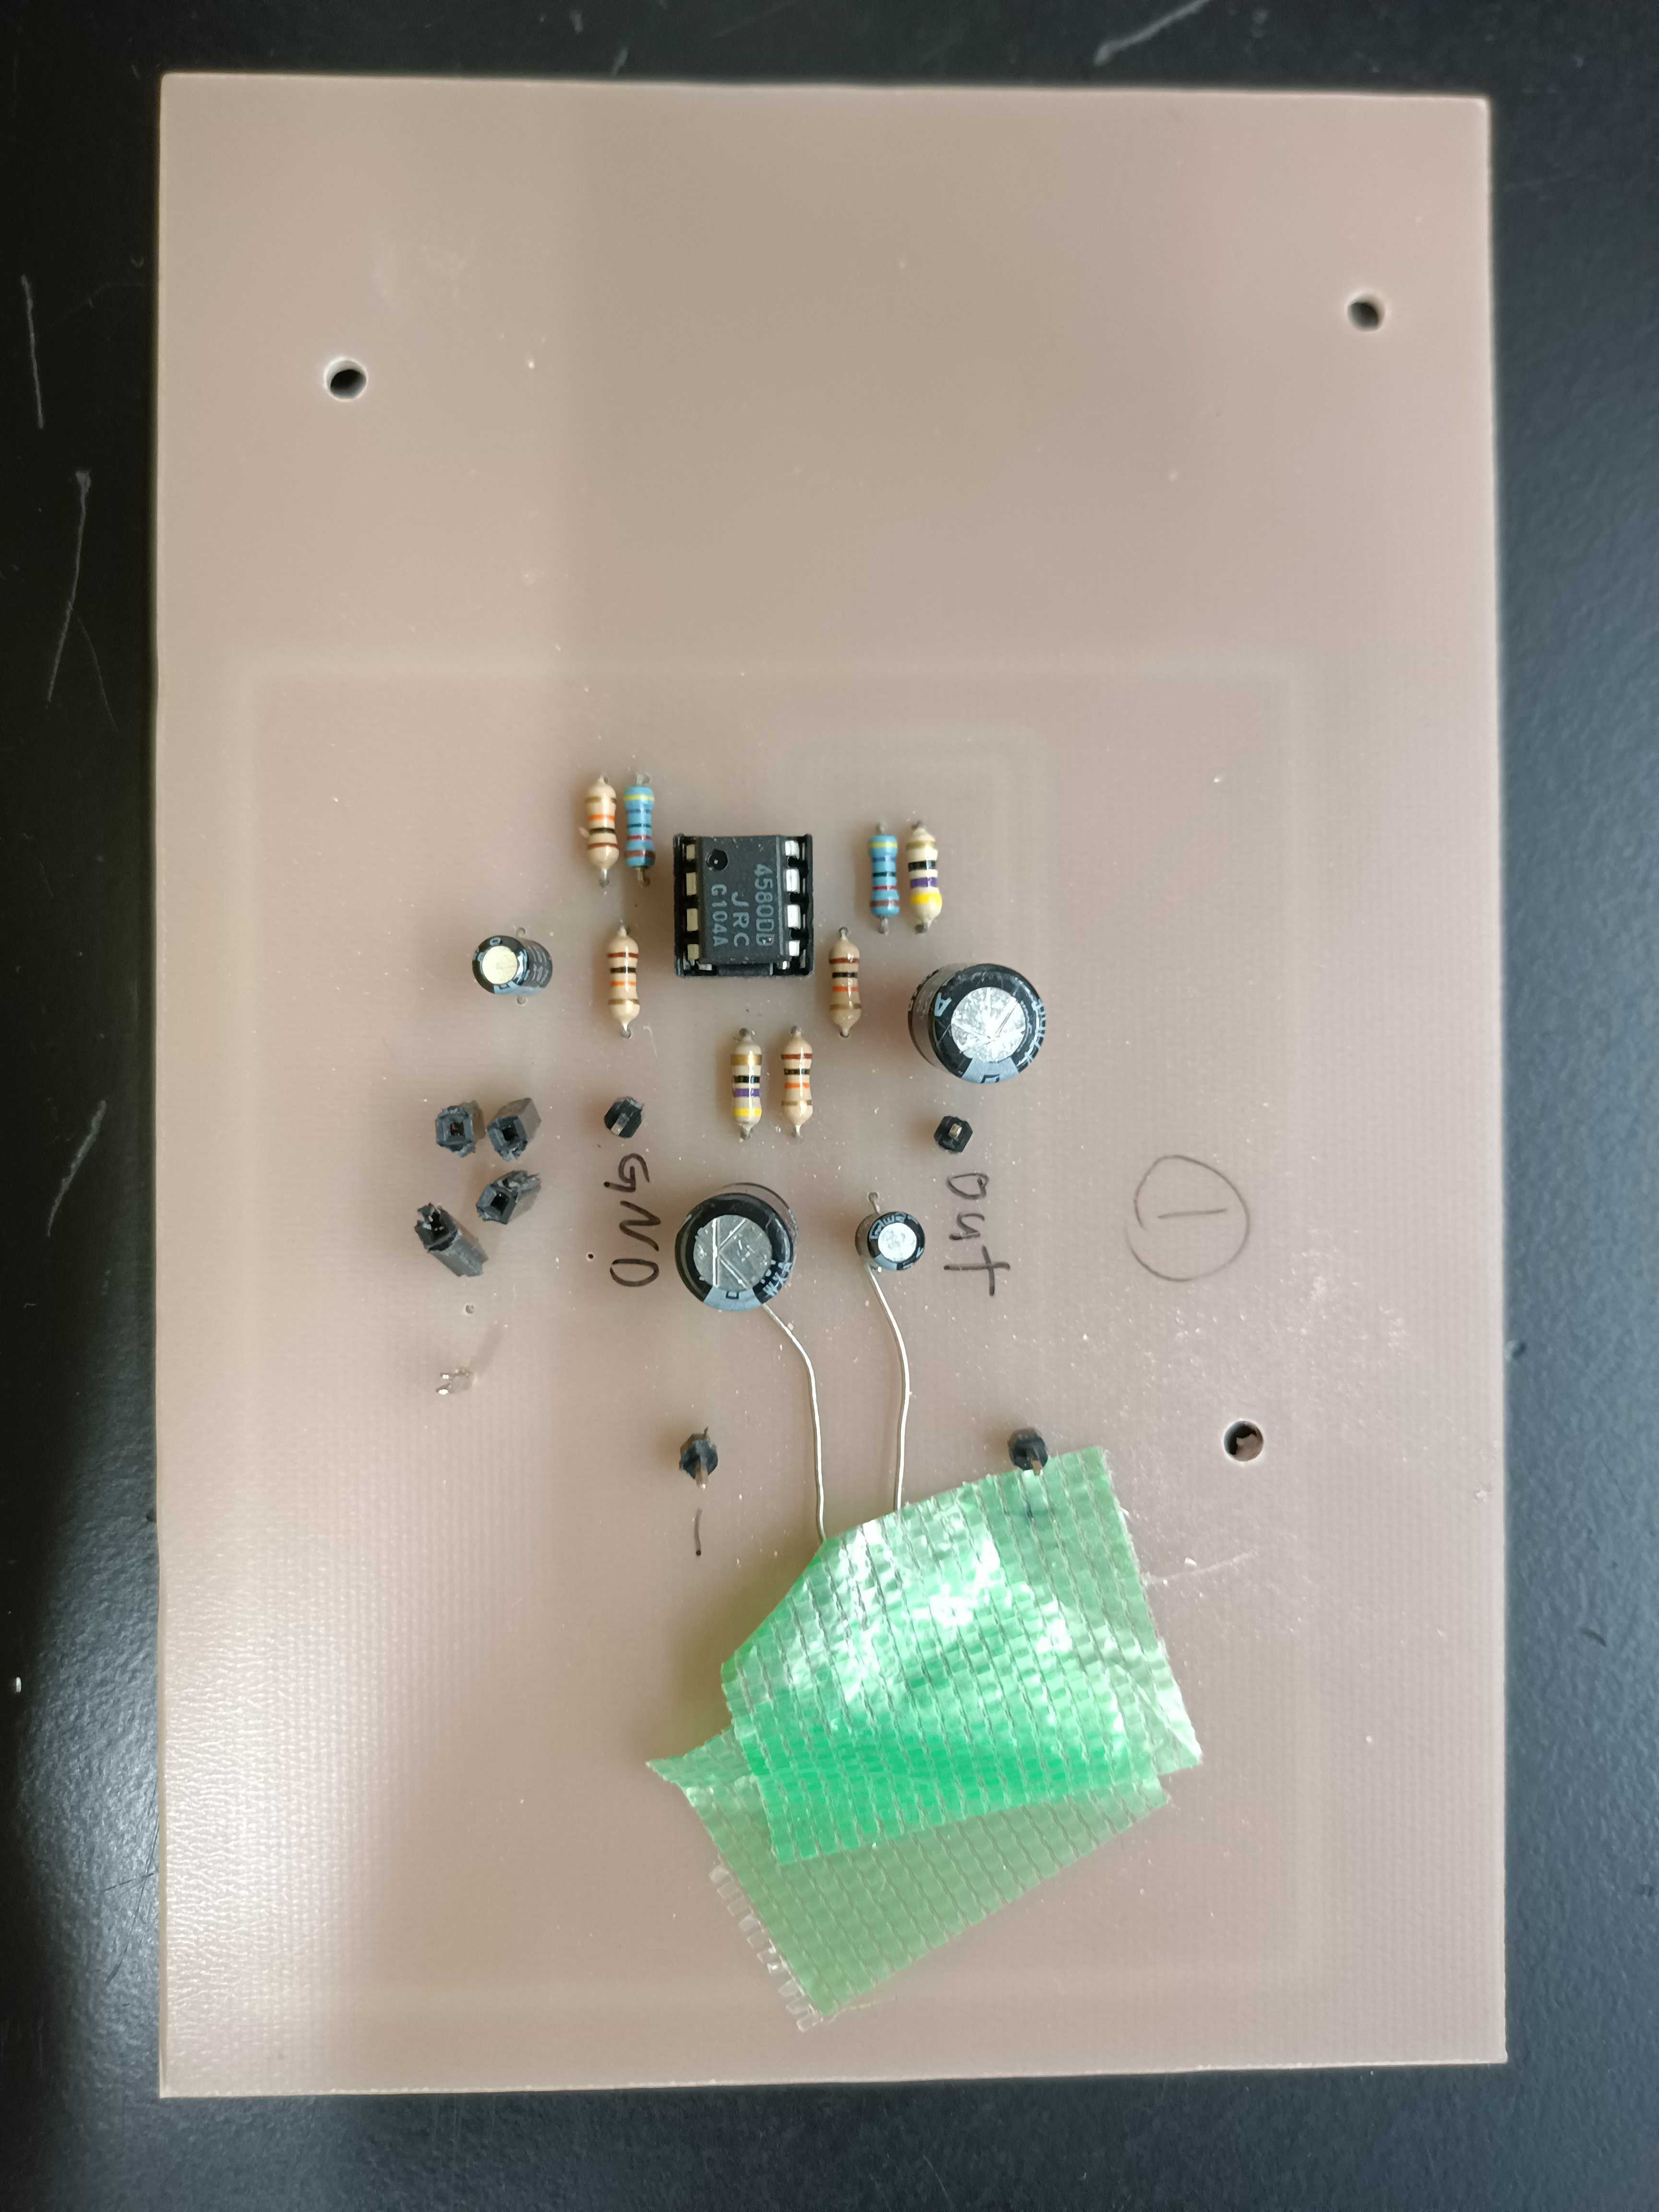
\includegraphics[width=8cm]{use/2.jpg}
		\caption{アンプ一台目}
		\label{fig:s_2}
	\end{minipage}
	\begin{minipage}[b]{0.5\linewidth}
		\centering
		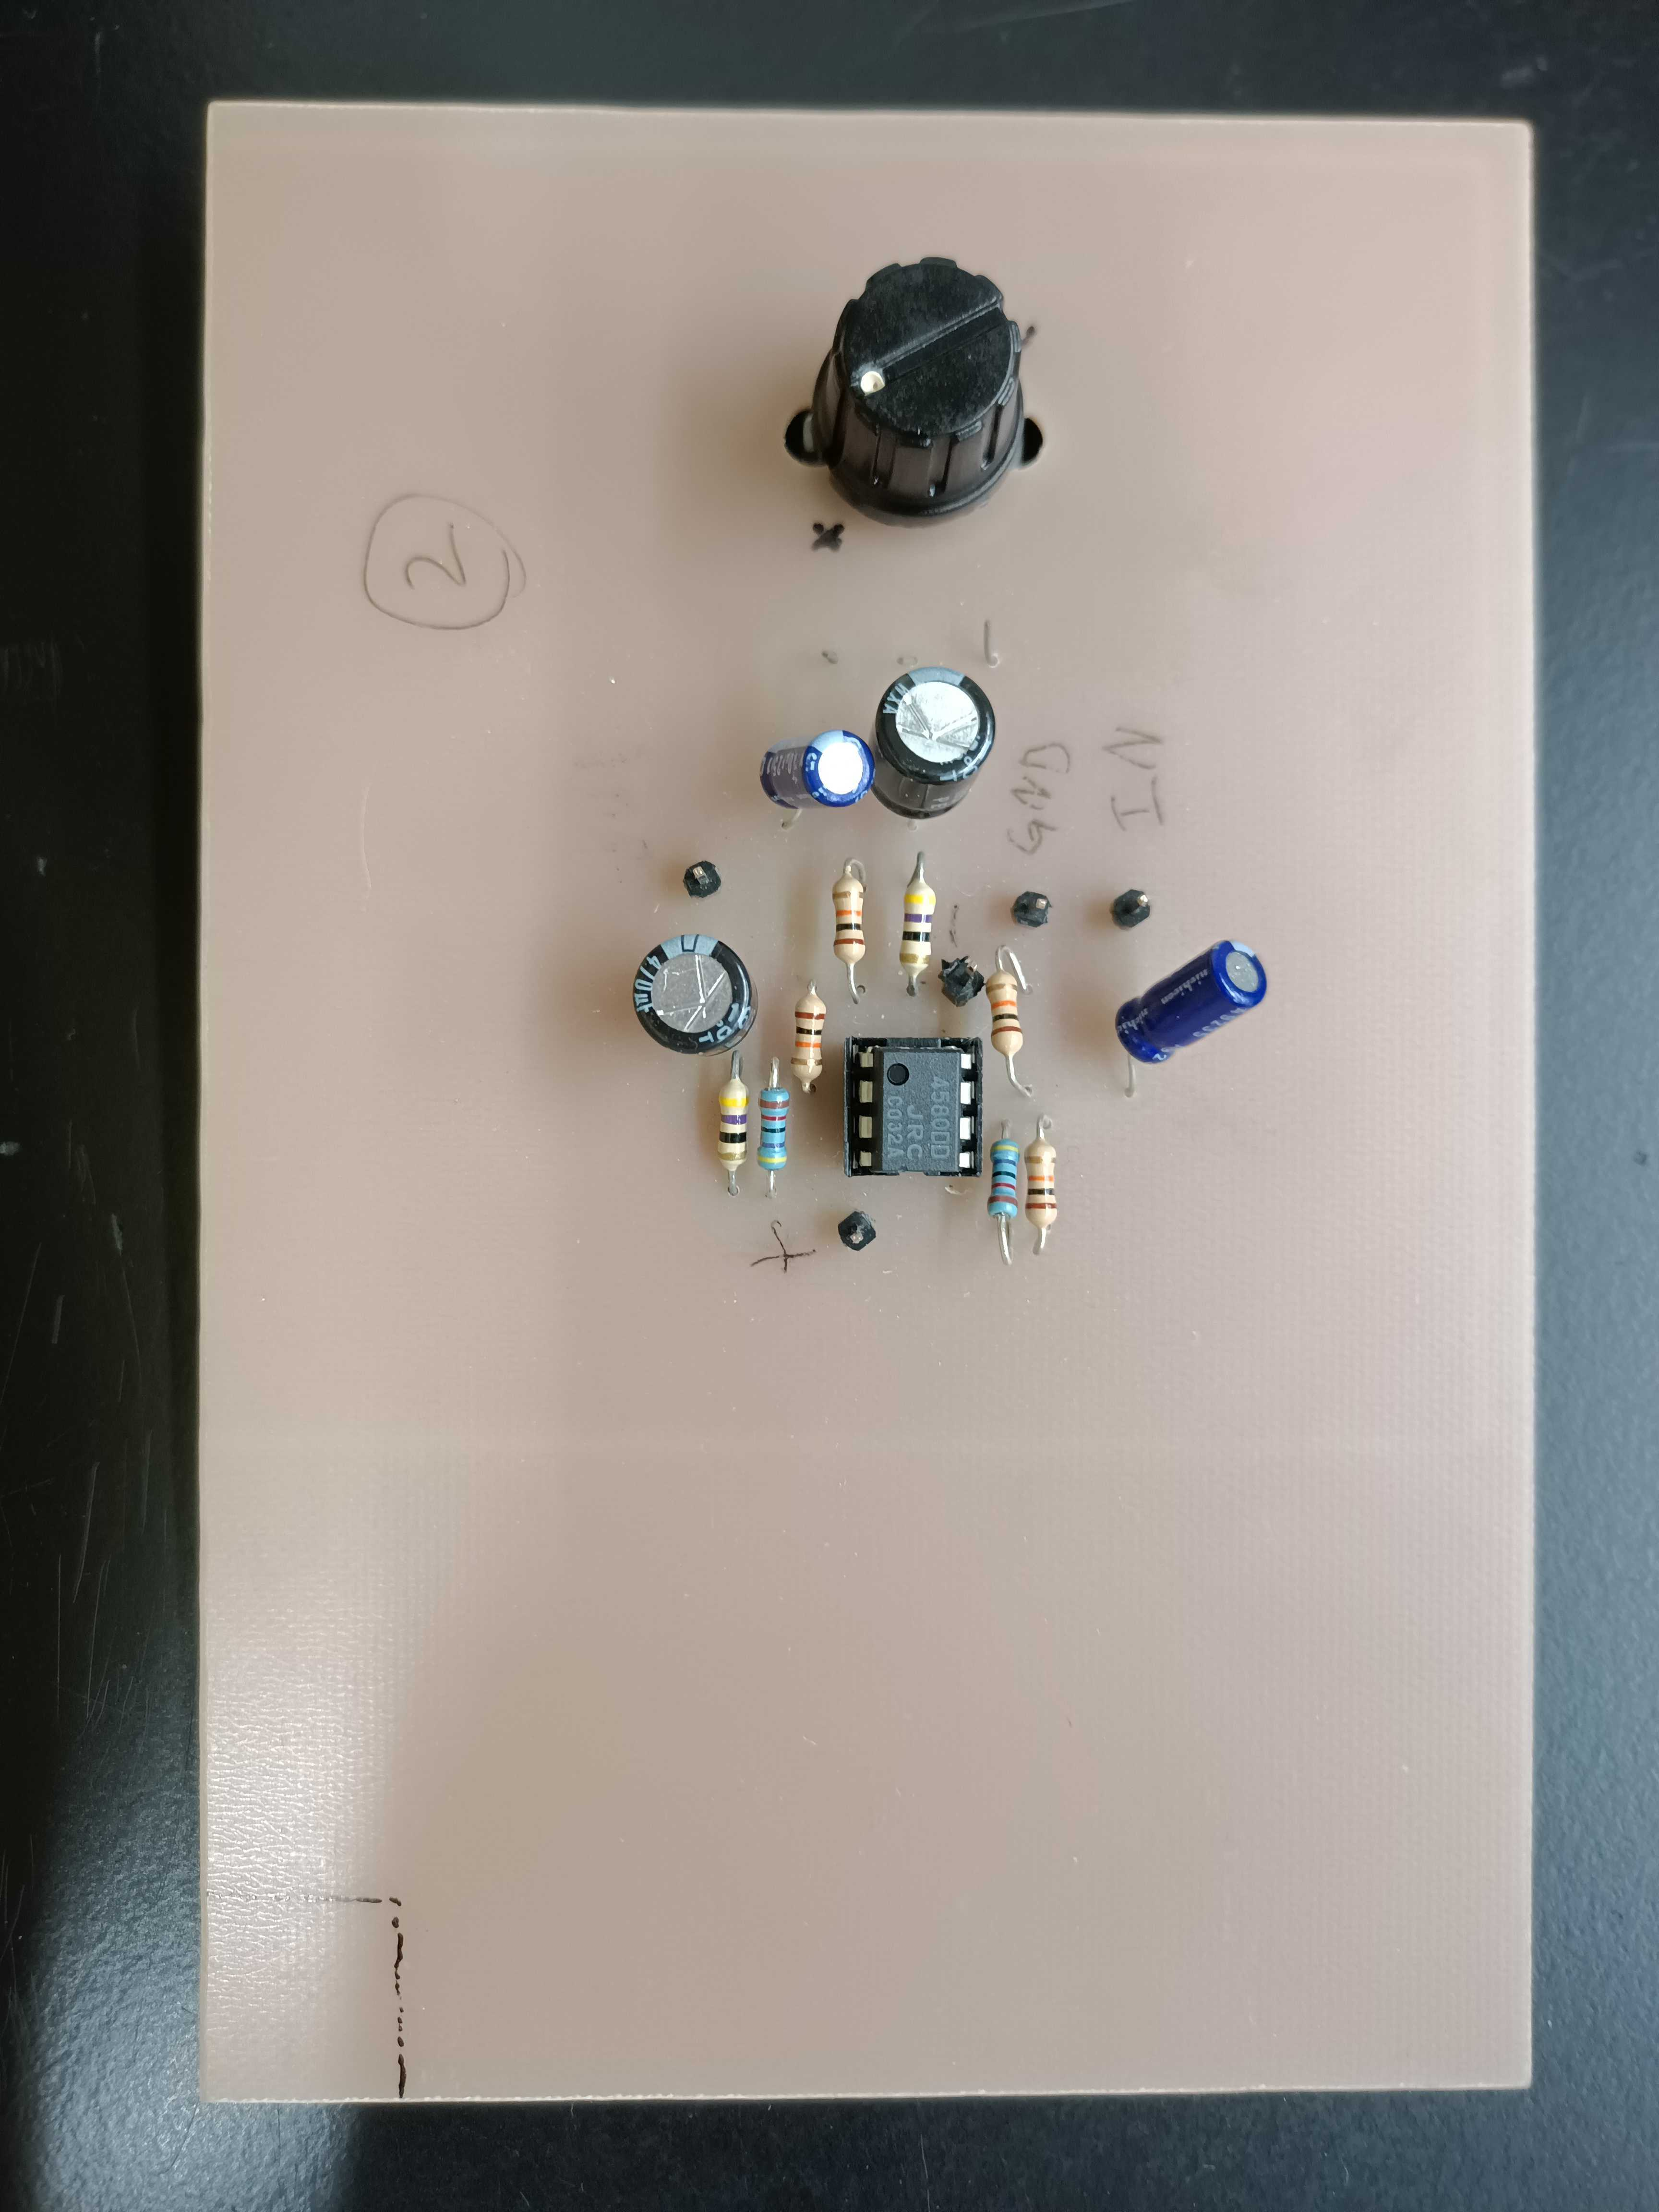
\includegraphics[width=8cm]{use/3.jpg}
		\caption{アンプ二台目}
		\label{fig:s_3}
	\end{minipage}
\end{figure}

\begin{figure}[H]
	\begin{minipage}[b]{0.5\linewidth}
		\centering
		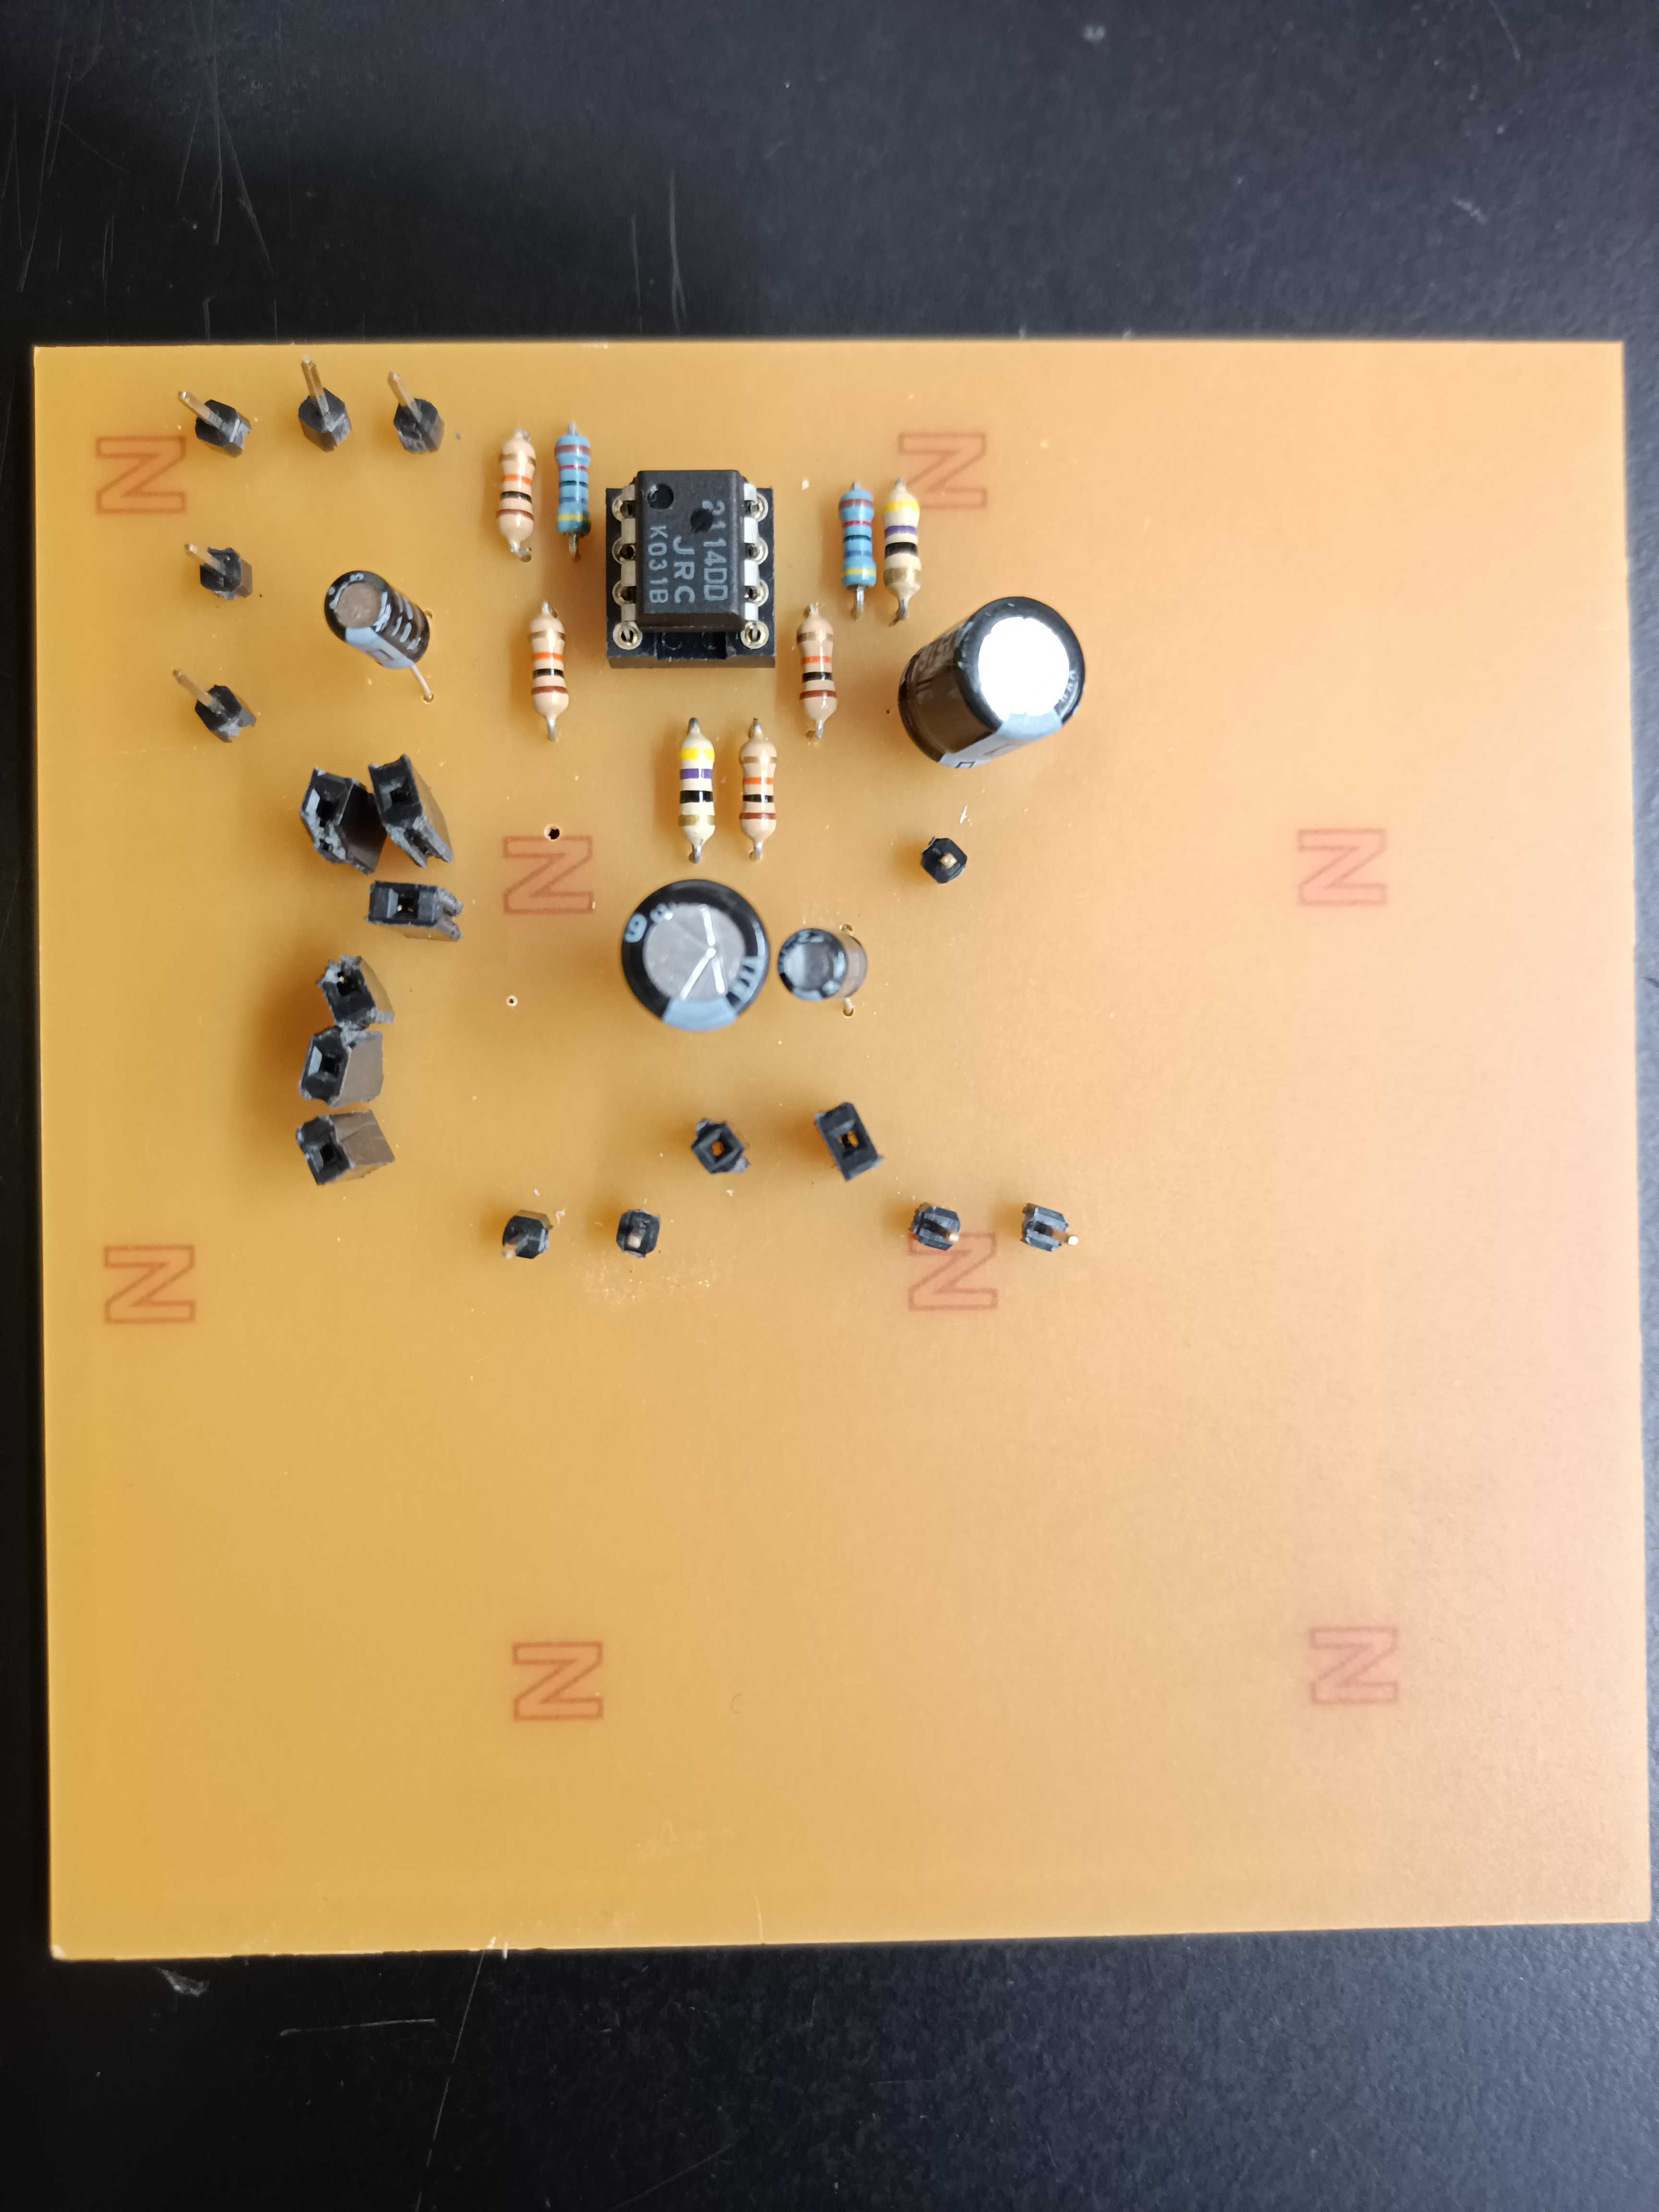
\includegraphics[width=8cm]{use/5.jpg}
		\caption{アンプ三台目}
		\label{fig:s_4}
	\end{minipage}
	\begin{minipage}[b]{0.5\linewidth}
		\centering
		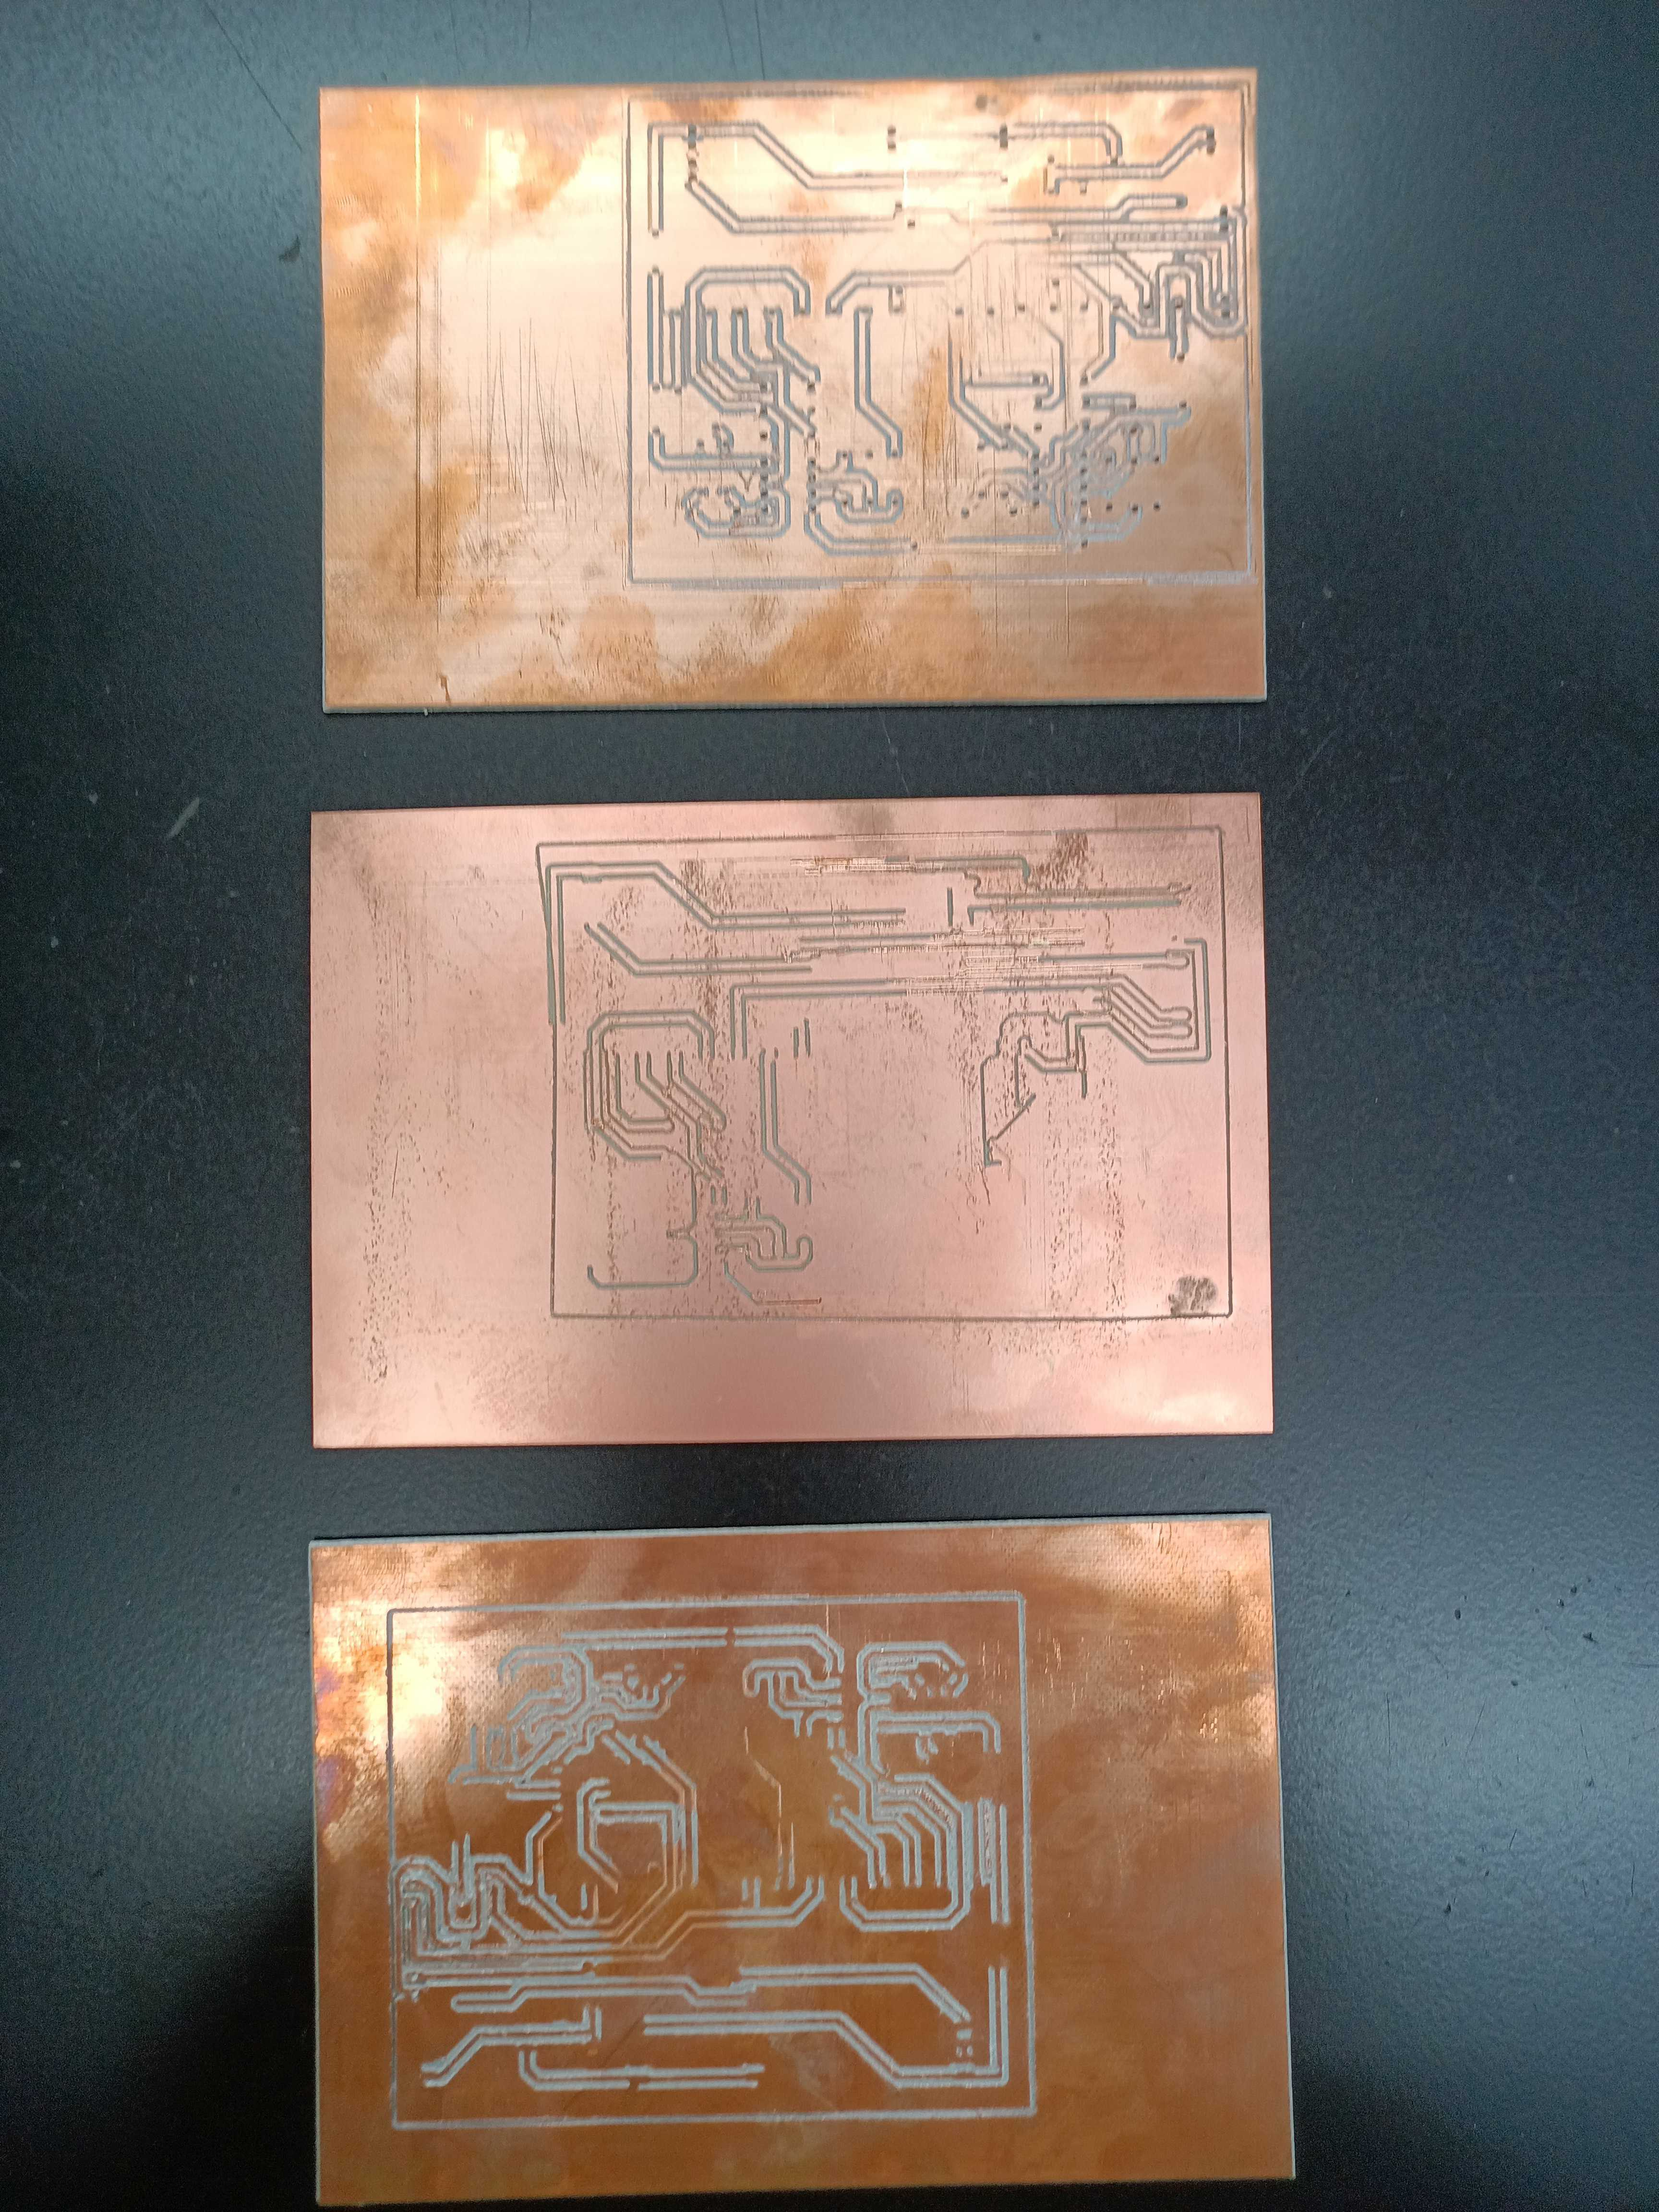
\includegraphics[width=8cm]{use/6.jpg}
		\caption{アンプ四代目になる予定だった残骸}
		\label{fig:s_5}
	\end{minipage}
\end{figure}

\begin{figure}[H]
	\begin{minipage}[b]{0.5\linewidth}
		\centering
		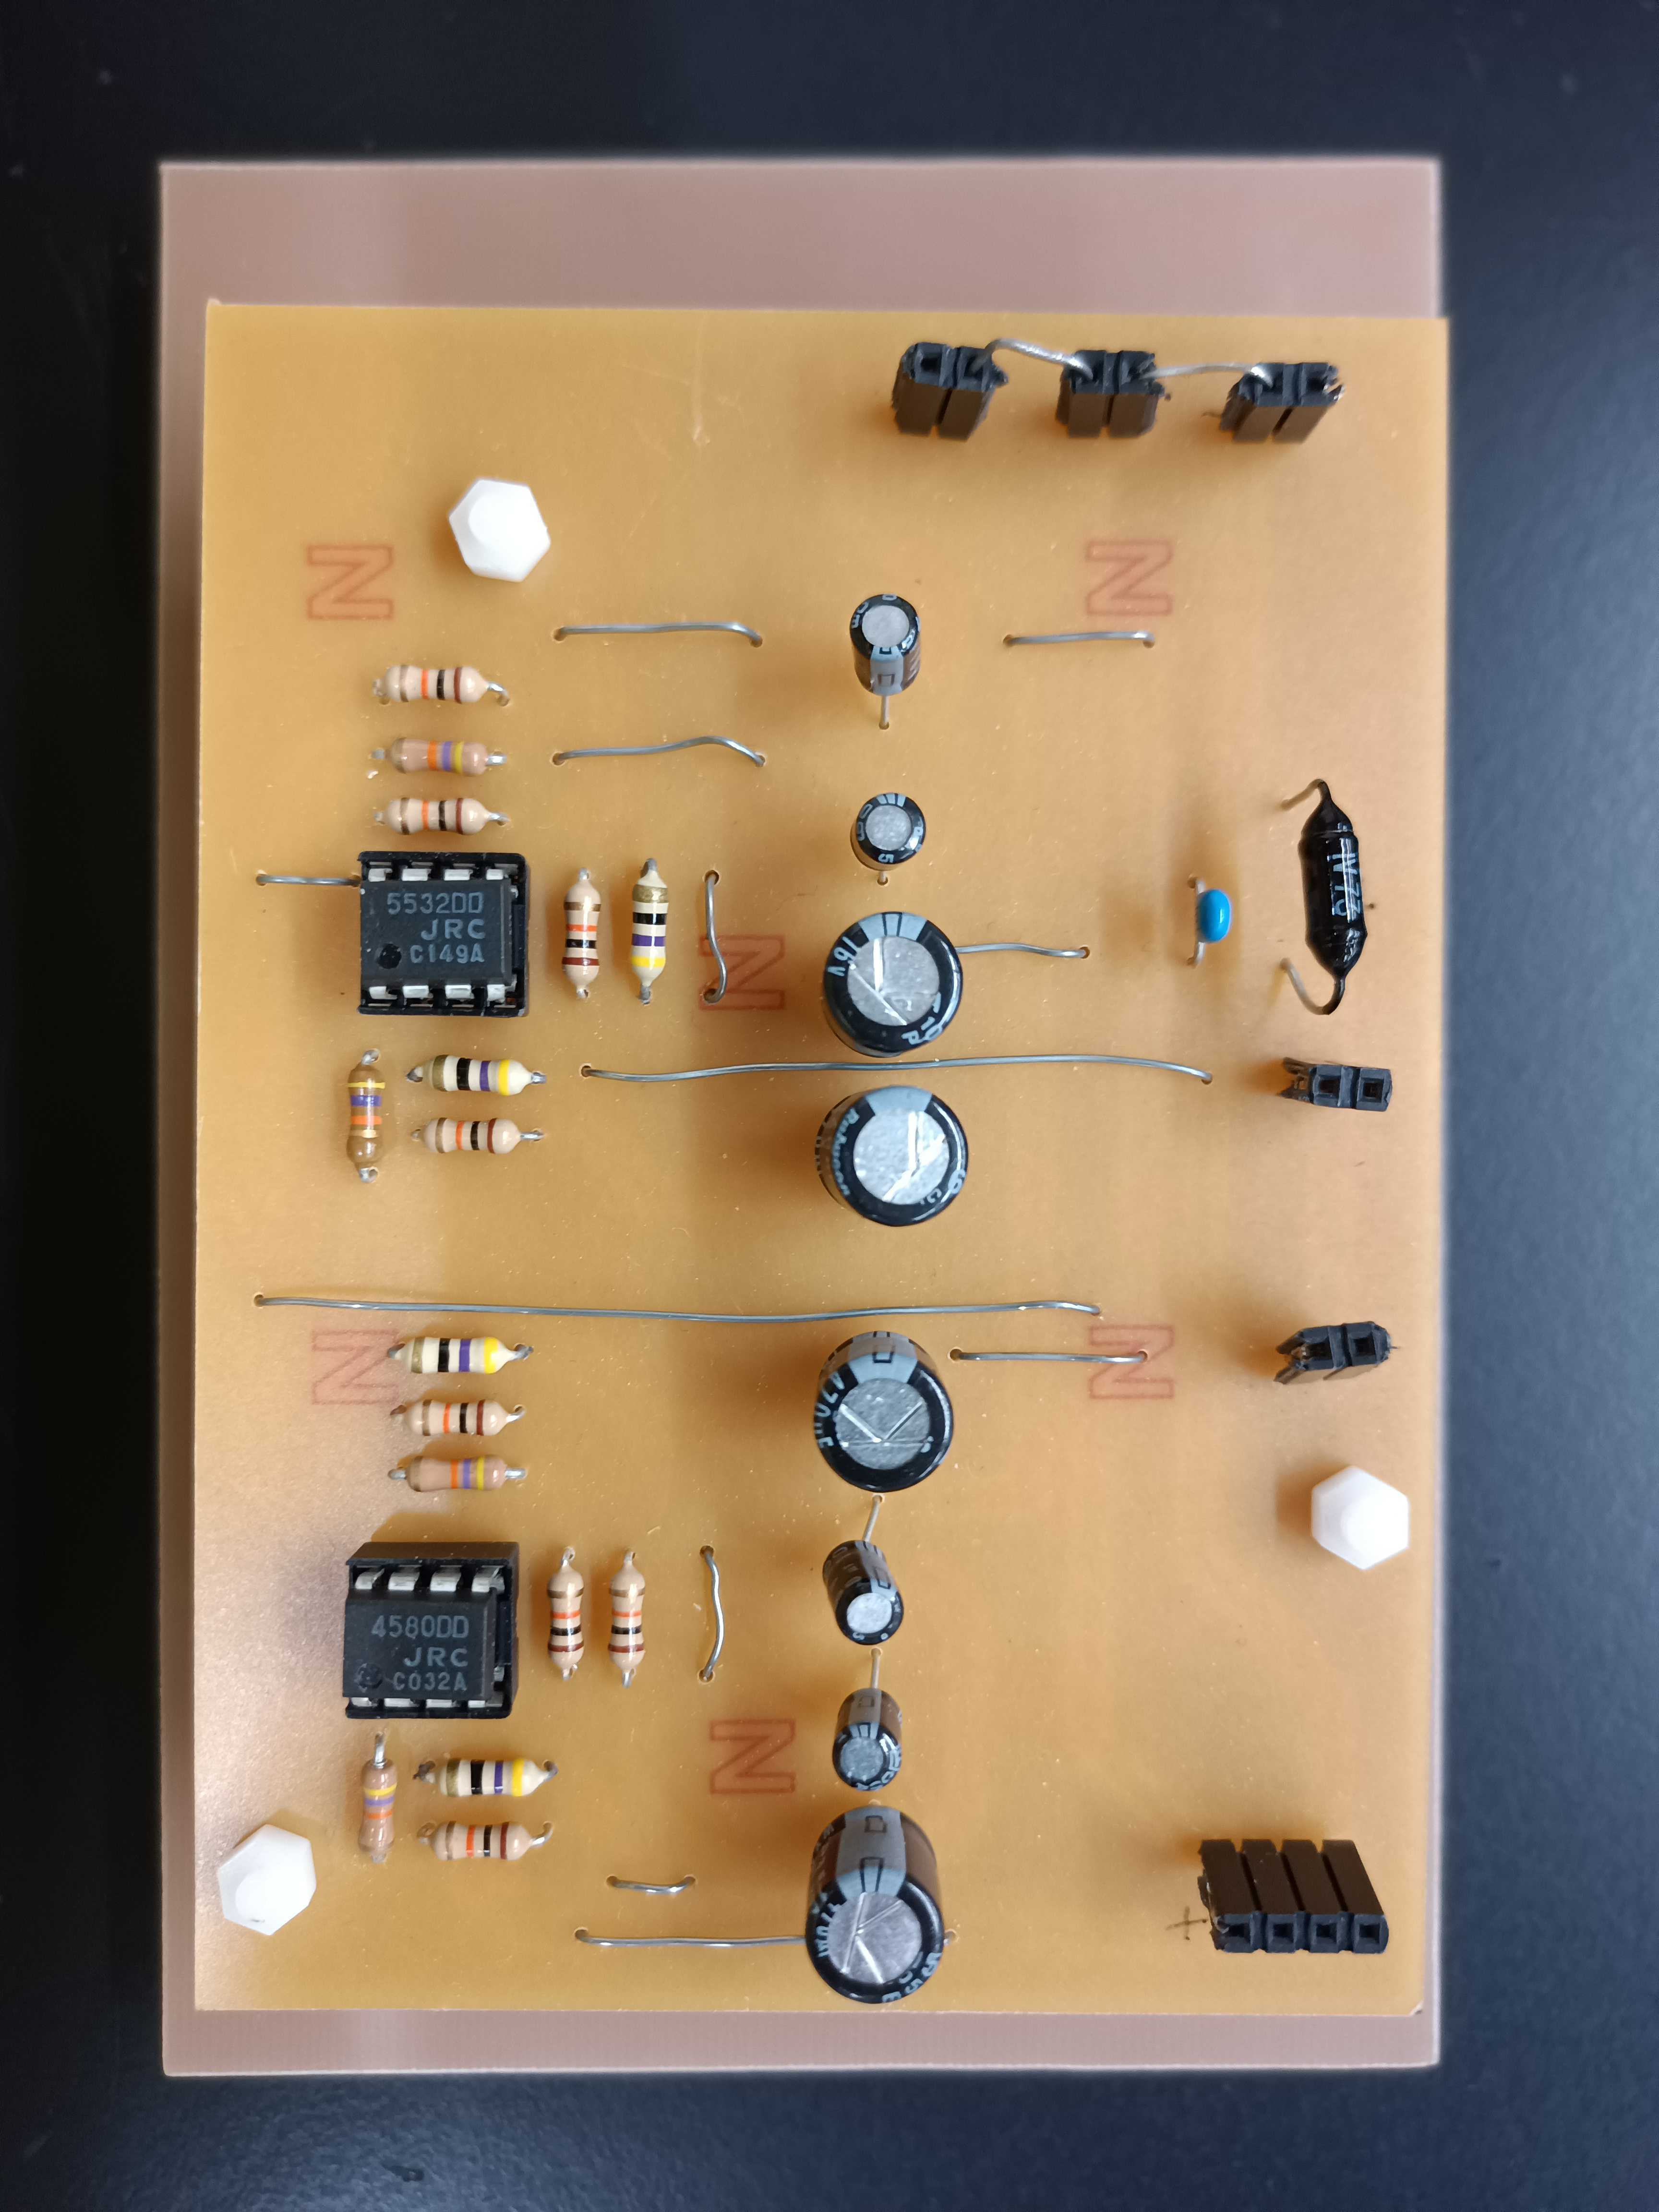
\includegraphics[width=8cm]{use/4.jpg}
		\caption{2号機アンテナの写真}
		\label{fig:s_6}
	\end{minipage}
	\begin{minipage}[b]{0.5\linewidth}
		\centering
		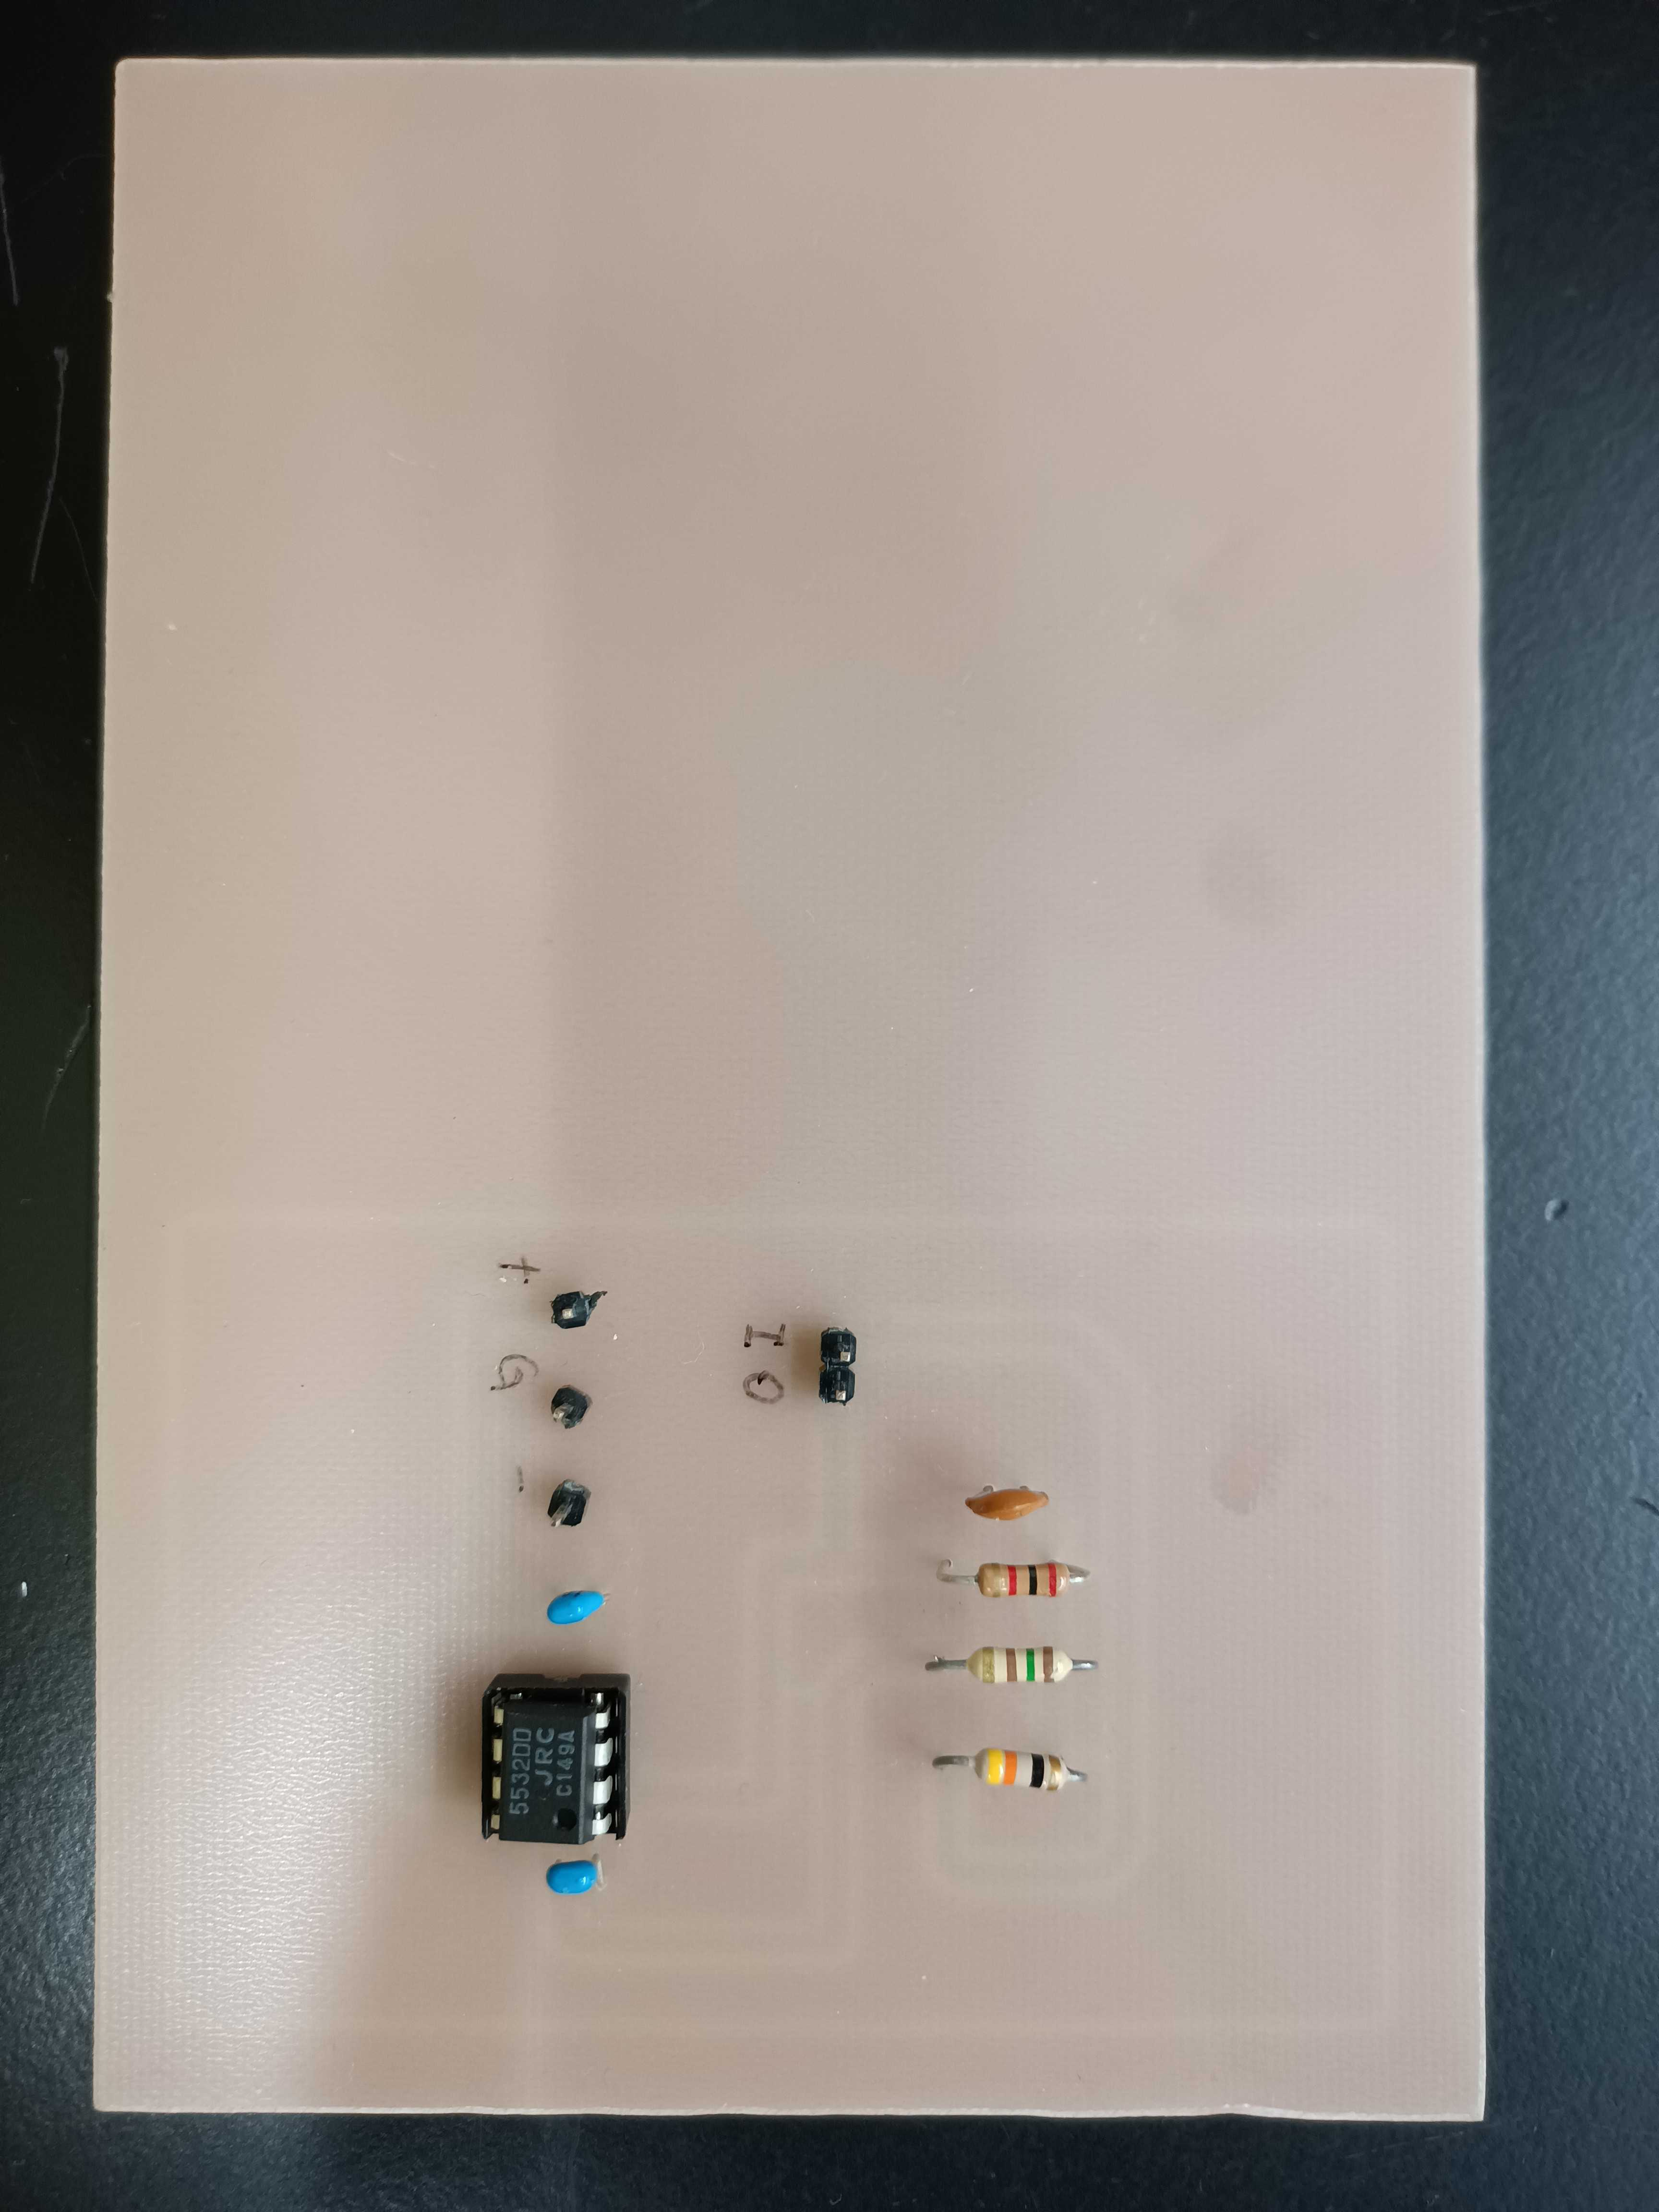
\includegraphics[width=8cm]{use/1.jpg}
		\caption{3号機アンテナの写真}
		\label{fig:s_7}
	\end{minipage}
\end{figure}

\subsection{役割分担}

役割分担で負担が偏ってしまった。

\end{document}
